% AKULIN R2 CP07 -- figure 6.8: source-landmark tracing, not a spectral fit.
% This is an editorial trace of the PUBLISHED contour, not reconstructed data.
% Independent broad shoulders, narrow-line peaks, four time markers, lower
% negative profile and the author's 55 cm^{-1} double-ended dimension preserved.
\documentclass[border=7pt]{standalone}
\usepackage{fontspec,unicode-math}
\setmainfont{Noto Serif}
\setmathfont{STIXTwoMath-Regular.otf}
\usepackage{tikz}
\usetikzlibrary{arrows.meta}
\tikzset{
 trace/.style={draw=black,line width=.88pt,line join=round,line cap=round},
 baseline/.style={draw=black,line width=.55pt},
 dim/.style={draw=black,line width=.5pt,{Latex[length=1.5mm,width=.85mm]}-{Latex[length=1.5mm,width=.85mm]}},
 lab/.style={font=\fontsize{11}{13.1}\selectfont,inner sep=.9pt},
 annot/.style={font=\fontsize{10.5}{12}\selectfont,inner sep=.7pt}
}
\begin{document}
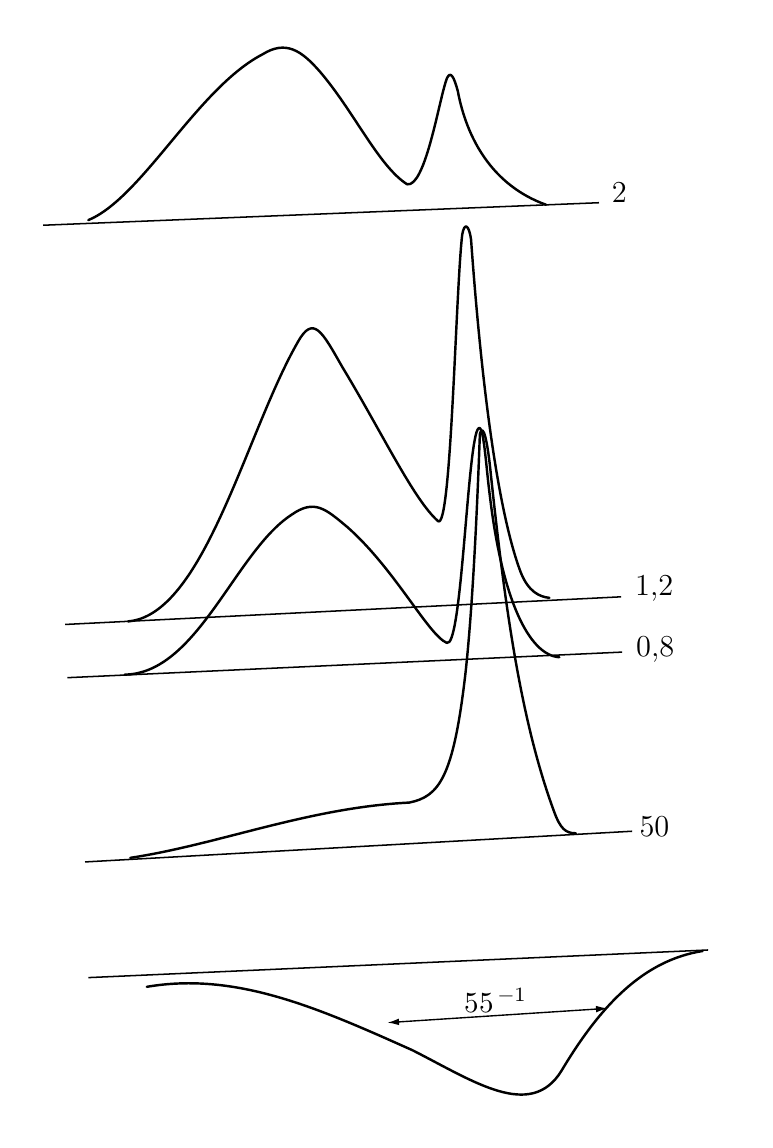
\begin{tikzpicture}[x=.014cm,y=-.013cm]
\path[use as bounding box] (0,-5) rectangle (650,1062);
% The author's baselines are mildly tilted in the printed reproduction.
\draw[baseline] (14,188)--(518,166);
\draw[trace] (55,183)
 .. controls (104,161) and (154,54) .. (213,21)
 .. controls (234,7) and (248,17) .. (265,38)
 .. controls (296,77) and (318,130) .. (344,148)
 .. controls (360,151) and (372,72) .. (379,48)
 .. controls (383,33) and (387,45) .. (390,57)
 .. controls (398,103) and (421,149) .. (470,168);
\node[lab,anchor=west] at (527,156) {2 мс};

\draw[baseline] (34,578)--(538,551);
\draw[trace] (91,575)
 .. controls (160,569) and (198,390) .. (245,302)
 .. controls (259,275) and (267,292) .. (285,326)
 .. controls (322,392) and (350,456) .. (372,477)
 .. controls (384,488) and (388,252) .. (394,197)
 .. controls (396,185) and (400,187) .. (402,202)
 .. controls (410,322) and (424,461) .. (447,527)
 .. controls (454,546) and (464,551) .. (473,552);
\node[lab,anchor=west] at (548,543) {1,2 мс};

\draw[baseline] (36,630)--(539,605);
\draw[trace] (88,627)
 .. controls (154,626) and (188,507) .. (239,471)
 .. controls (260,455) and (270,465) .. (290,483)
 .. controls (333,524) and (363,588) .. (380,596)
 .. controls (393,602) and (398,421) .. (407,390)
 .. controls (413,372) and (415,419) .. (419,452)
 .. controls (430,552) and (454,608) .. (482,610);
\node[lab,anchor=west] at (549,602) {0,8 мс};

\draw[baseline] (52,810)--(548,780);
\draw[trace] (93,806)
 .. controls (173,793) and (254,757) .. (346,752)
 .. controls (373,746) and (386,728) .. (397,625)
 .. controls (404,556) and (408,451) .. (410,392)
 .. controls (413,380) and (417,399) .. (420,432)
 .. controls (432,553) and (446,669) .. (477,760)
 .. controls (483,778) and (488,782) .. (497,782);
\node[lab,anchor=west] at (552,776) {50 мкс};

% Below is an absorption-like negative dip (author's schematic), not a measured array.
\draw[baseline] (55,923)--(617,896);
\draw[trace] (108,932)
 .. controls (189,917) and (264,953) .. (349,994)
 .. controls (404,1024) and (456,1063) .. (484,1014)
 .. controls (520,949) and (559,906) .. (612,897);
% The double arrow indicates the printed relative separation (55 cm^{-1}),
% not a numerically calibrated x-axis; tips must stay on distinct locations.
\draw[dim] (326,967)--(526,953);
\node[annot,anchor=south] at (425,960) {$55\,\mathrm{см}^{-1}$};
\end{tikzpicture}
\end{document}
